\mychapter{implementation}{Implementation/realization - cloudml-engine}

In the previous chapter the design of CloudML was introduced.
In this chapter the implementation of this design will be presented and described.
First section is a technical overview of some of the general solutions within 
the implementation.
The rest of the chapter is split into different sections, one for each important part of the implementation.
Topics are about
\begin{ii}
  \iitem submodules and their tasks,
  \iitem the depdency system,
  \iitem communication with cloud providers,
  \iitem \myac{M@RT} through actor model and
  \iitem data serialization.
\end{ii}

\mysection{technologies}{Technology overview}

CloudML is implemented as a \emph{proof-of-concept} framework~\cite{cloudml-engine}
(from here known as \emph{cloudml-engine}). 
The implementation, \emph{cloudml-engine}, 
is based on \emph{state-of-the-art} technologies that appeal to the academic community.
Technologies chosen for \emph{cloudml-engine} are not of great importance to the concept of CloudML itself,
but it is still important to understand which technologies are chosen, what close alternatives exists
and why they are chosen.

\paragraph{Language and environment.} 

The importance of a \emph{programming language} and \emph{environment} were
described in \citesec{technological-assessments}.
These are core ideas to fulfill \citereq{foundation}, emphasizing the importance of a strong foundation.
Here is a list describing some of the languages and environments considered:
\begin{description}
  \item[Java (\myac{JVM}).] Well known and recognized in both the enterprise domain, as well as the academic world.
    Support object-oriented programming and a vast amount of libraries are supported by the \myac{JVM}.
  \item[JavaScript (Node.js).] A newer and unfamiliar type of technology which has yet to 
    make a large footprint in the two domains. 
    It is based on the \myac{JIT}-powered JavaScript engine V8 created by Google and follows a 
    CommonJS-based module pattern over an event-driven architecture.
  \item[Scala (\myac{JVM}).] Same environment as Java, 
    but a more modern language which focuses and supports both 
    object-oriented programming and functional programming.
    This language is gaining popularity among both the academic and enterprise domain.
    Libraries supported by Java are also supported by Scala.
  \item[Python.] Well known in the academic world. Follows both object-oriented and functional programming as
    Scala.
  \item[C\# (.NET).] Language and environment by Microsoft.
\end{description}
Languages in this list are introduced because of their overall popularity.
Some were introduced despite this, such as \emph{Node.js}, 
which is brought in as an consideration because of the abilities to operate
with \myac{JSON}, cloud interaction and modernity.

Based on these considerations Scala is a good choice, it fulfills the core ideas and match
the requirement \citereq{foundation}:
\begin{itemize} 
  \item \myac{JVM} is a popular platform, and then especially Java.
  \item Compatible with Java and libraries written in Scala can be interacted with by Java as well.
  \item The reason not to use plain Java is because Scala is an appealing state-of-the-art language.
  \item Emphasizes on functional programming which is leveraged in the implementation.
  \item Built in system for actor model~\cite{actors:haller07}, which is utilized in the implementation.
\end{itemize}
Based on these benefits Scala is chosen, and \emph{cloudml-engine} is written in this language.

\paragraph{Automatic build system.}

There are two main methods used to automatically build Scala programs, 
either using a Scala-specific tool called \myac{SBT} or a more general tool called Maven. 
For \emph{cloudml-engine} to have an academic appeal it is essential to choose the technology
with most closeness to Java, hence Maven is the best option.
More about the module dependencies in \citesec{dependencies}.

\mysection{modules}{Modules and application flow}
\begin{figure}[tb]
  \begin{center}
    \begin{minted}[mathescape,
                   linenos,
                   numbersep=5pt,
                   gobble=2,
                   frame=lines,
                   framesep=2mm]{xml}

  <repositories>
   <repository>
    <id>cloudml-engine</id>
    <url>
     https://repository-eirikb.forge.cloudbees.com/release
    </url>
   </repository>
  </repositories>
  <dependencies>
   <dependency>
    <groupId>no.sintef</groupId>
    <artifactId>engine</artifactId>
    <version>0.1</version>
   </dependency>
  </dependencies>
    \end{minted}
  \end{center}
  \caption{Example Maven conficuration section to include cloudml-engine.}
  \label{fig:pom-example}
\end{figure}



\emph{Cloudml-engine} is divided into four main modules~(\citefig{cloudml-engine}).
This is to distribute workload and divide \emph{cloudml-engine} into logical parts for each task.

\paragraph{Engine.} 

\begin{figure}[tb]
  \begin{center}
    \begin{minted}[mathescape,
                   linenos,
                   numbersep=5pt,
                   gobble=2,
                   frame=lines,
                   framesep=2mm]{scala}

  import no.sintef.cloudml.engine.Engine
  ...
  val runtimeInstances = Engine(account, List(template))
    \end{minted}
  \end{center}
  \caption{Example client (Scala) callout to cloudml-engine.}
  \label{fig:cloudml-engine-usage}
\end{figure}



\begin{figure}[tb]
  \begin{center}
    \subfigure[Application modules]{
      \begin{tikzpicture}[scale=0.8, transform shape]
        \node (AuxNode01) [text width=4cm] {};
        \node (Engine) [class, left=of AuxNode01, rectangle split, rectangle split parts=2] { 
          \textbf{Engine} 
          \nodepart{second}Entry point. Orchestration.
        };
        \node (AuxNode02) [left=of Engine] {};
        \node (Kernel) [class, below=of AuxNode01, rectangle split, rectangle split parts=2] { 
          \textbf{Kernel} 
          \nodepart{second}Node domains. Converts JSON to Node Entities.
        };
        \node (Repository) [class, above=of AuxNode01, rectangle split, rectangle split parts=2] { 
          \textbf{Repository} 
          \nodepart{second}Instance domains. Convert Nodes to Instances.
        };
        \node (Cloud-Connector) [class, right=of AuxNode01, rectangle split, rectangle split parts=2] { 
          \textbf{Cloud-Connector} 
          \nodepart{second}Connects to providers (jclouds).
        };

        \draw [arrow] (Engine) -- (Kernel);
        \draw [arrow] (Engine) -- (Cloud-Connector);
        \draw [arrow] (Engine) -- (Repository);
        \draw [arrow] (Cloud-Connector) -- (Kernel.east);
        \draw [arrow] (Cloud-Connector) -- (Repository.east);
        \draw [arrow] (Repository) -- (Kernel);
        \draw [extend] (AuxNode02) -- (Engine);
      \end{tikzpicture}
    }

    \subfigure[Legend]{
      \begin{tikzpicture}[scale=0.7, transform shape]
        \node (Module) [class, label=below:Application modules] { Module };

        \node (AuxNode01) [right=of Module] {};
        \node (AuxNode02) [right=of AuxNode01] {};
        \node (AuxNode03) [right=of AuxNode02] {};
        \node (AuxNode04) [right=of AuxNode03] {};

        \draw[arrow] (AuxNode01) -- node[below] {Dependency} (AuxNode02);
        \draw[extend] (AuxNode03) -- node[below] {Entry} (AuxNode04);
      \end{tikzpicture}
    }
  \end{center}
  \caption{Architecture of cloudml-engine}
  \label{fig:cloudml-engine}
\end{figure}

\begin{figure}

  \begin{center}
    \begin{tikzpicture}
      \stickman{head}
      \node[below of=head, text width=2cm] (Body) {};

      \node[box, right=of head, minimum width=3.8cm, minimum height=3.5cm, xshift=1cm, yshift=-1.5cm] (System) {};
      \node[box, right=of head, xshift=2cm, yshift=-0.7cm] (Engine) {Engine};
      \node[box, below=of Engine, yshift=0.5cm] (Cloud-Connector) {Cloud-Connector};
      \node[box, below=of Cloud-Connector, yshift=0.5cm] (RuntimeInstance) {RuntimeInstance};

      \node (Rackspace) [tcloud, right=of System, xshift=0.5cm, yshift=1.5cm] {Rackspace};
      \node (EC2) [tcloud, below=of Rackspace] {EC2};

      \draw[arrow] (Body.east) -- (Engine.west);
      \draw[arrow] (Engine.south) -| (Cloud-Connector.north);

      \draw[arrow] (Cloud-Connector.east) -- (Rackspace.west);
      \draw[arrow] (Cloud-Connector.east) -- (EC2.west);

      \draw[arrow] (Cloud-Connector.south) -| (RuntimeInstance.north);
      \draw[arrow] (RuntimeInstance.west) -- (Body.east);

      \node (Label01) [below=of Body, yshift=-1.5cm] {User};
      \node (Label02) [right=of Label01, xshift=1.2cm] {Cloudml-engine};
      \node [right=of Label02, xshift=1.2cm] {Cloud providers};

    \end{tikzpicture}
  \end{center}
  \caption{Usage flow in cloudml-engine}
  \label{fig:cloudml-engine-flow}
\end{figure}


The main entry point to the application, this is a Scala Object used to initialize provisioning.
Interaction between \texttt{user} and \texttt{Engine} is visible in \citefig{cloudml-engine-flow} 
where the user will initialize provisioning by calling \texttt{Engine}.
\texttt{Engine} will also do orchestration between the three other modules
as shown in \citefig{cloudml-engine}.
Since \texttt{Cloud-Connector} is managed by \texttt{Engine} other actions against 
instances are done through \texttt{Engine}.
The first versions of \emph{cloudml-engine} did not use \texttt{Engine} as orchestrator but
instead relied on each module to be a sequential step, this proved to be harder to maintain
and also introduced cyclic dependencies.

\paragraph{Kernel.} 

\texttt{Kernel} contains CloudML specific entities such as Node and Template.
The logical task of \texttt{Kernel} is to map \myac{JSON} formatted strings to 
\texttt{Templates} including \texttt{Nodes}.
This is some of the core parts of the \myac{DSL}, hence it is called \emph{\texttt{Kernel}}.
\texttt{Accounts} are separate parts that are parsed equally as \texttt{Templates},
 but by another method call. All this is transparent for users as all data will
be provided directly to \texttt{Engine} which will handle the task
of calling \texttt{Kernel} correctly.

\paragraph{Repository.} 

Has \texttt{Instance} entities, these are equivalent to \texttt{Nodes} in \texttt{Kernel},
but are specific for provisioning. Repository will do a mapping from \emph{Nodes} (including \emph{Template})
to \emph{Instances}. Future versions of \texttt{Repository} will also do some logical superficial validation
against \emph{Node} properties, for instance at the writing moment it is not possible to 
demand LoadBalancers on Rackspace for specific geographical locations.

\mysection{dependencies}{Internal and external dependencies}
\begin{figure}[tb]
  \subfigure[dependency-graph-without-test] {
    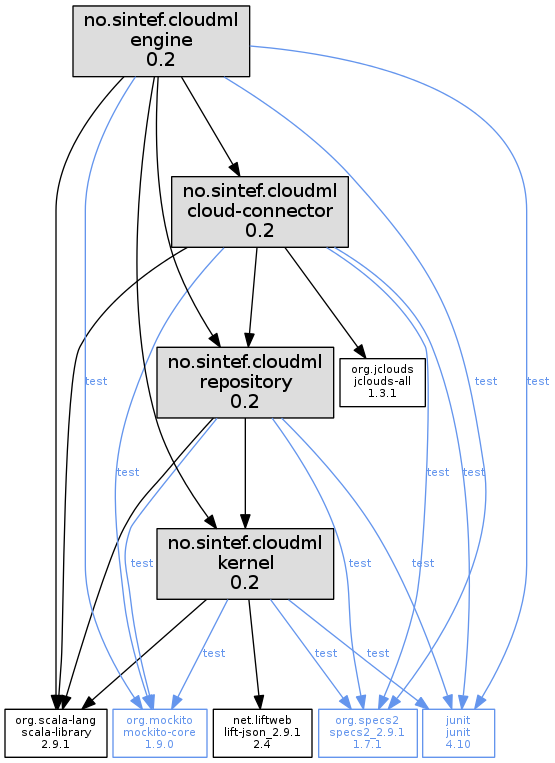
\includegraphics[width=8cm]{imgs/dependency-graph-2.png}
    \label{fig:dependency-graph-without-test}
  }
  \subfigure[dependency-graph-with-test] {
    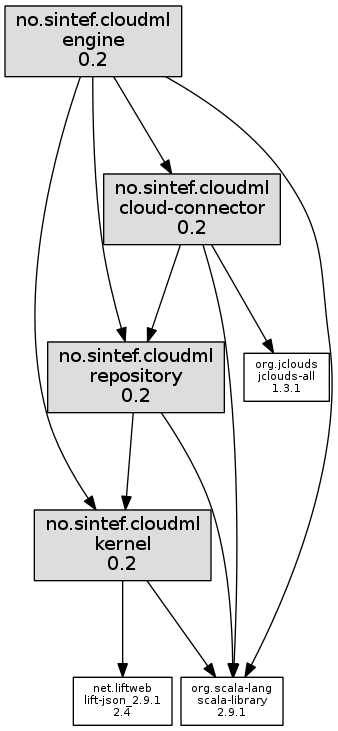
\includegraphics[width=5cm]{imgs/dependency-graph-1.png}
    \label{fig:dependency-graph-with-test}
  }
  \caption{Maven dependency graph (with and without test scope).}
  \label{fig:dependency-graph}
\end{figure}


Maven support modules which were used to split \emph{cloudml-engine} into the appropriate 
modules as shown in~\citefig{cloudml-engine}. 
The dependency system in Maven between modules is used to match the dependencies outlined in~\citefig{cloudml-engine}.
Parts of a dependency reference in a Maven configuration can be seen in~\citefig{pom-example},
although this is not dependency management in between \emph{cloudml-engine} modules but rather
how to add \emph{cloudml-engine} as a dependency itself.

\section{Cloud connection}

The module bridging between \emph{cloudml-engine} and providers.
It does not contain any entities, and only does logical code. 
It is built to support several libraries and interface these. At the moment it only implements the earlier
mentioned library jclouds.

The bridge between \emph{cloudml-engine} and cloud providers is an important aspect of the application, 
and as a requirement it is important to use an existing library to achieve this connection.
Some libraries have already been mentioned in the \emph{APIs} section in~\citechap{state-of-the-art},
of these only \emph{jclouds} is based on Java-technologies and therefore suites \emph{cloudml-engine}.
Jclouds uses Maven for building as well, and is part of Maven central which makes 
it possible to add jclouds directly as a module dependency.
Jclouds contains a template system which is used through code directly, this is utilized 
to map CloudML templates to jclouds templates.

\hr

Cloudml-engine use jclouds.org library to connect with cloud providers, giving it support
for 24 providers out of the box to minimize \emph{complexity} as well as stability and \emph{robustness}.

\section{Actor model}

Actors ~\cite{actors:haller07}.
With this asynchronous solution CloudML got concurrent communication with nodes under provisioning.
The model is extended by adding a callback-based pattern allowing each node to provide 
information on property and status changes.
Developers exploring the implementation can then choose to ``listen'' for updating events from each node,
and do other jobs / idle while the nodes are provisioned with the actors model.
The terms are divided for a node before and under provisioning, the essential is to introduce 
\emph{M@RT} to achieve a logical separation.

\hr

As mentioned earlier \emph{cloudml-engine} utilizes the actors model through Scala,
this approach is used to achieve asynchronous provisioning.
This is important as provisioning can consume up to minutes for each instance.
Beside the standard model provided by Scala \emph{cloudml-engine} uses
a callback-based pattern to inform users of the library when instance statues
are updated and properties are added.

\section{From text to objects}
\begin{table}
  \begin{tabular*}{\textwidth}{@{\extracolsep{\fill}}| l | l | l | l |}
      \hline
        \textbf{Requirement} & 
        \textbf{XML} & 
        \textbf{JSON} &
        \textbf{YAML} \\
      \hline
        Community & $2$ & $2$ & $1$ \\ \hline
        Technology support & $2$ & $2$ & $1$ \\ \hline
        Human-readable & $1$ & $2$ & $3$ \\ \hline
        Web-service friendly & $2$ & $2$ & $0$ \\ \hline
  \end{tabular*}
  \caption{Comparing lexical formats (\citesec{technological-assessments})
    with aspects from requirement \citereq{lexical-template}.
    Weighting from zero ($0$) to three ($3$) respectively least to most supported.}
  \label{table:requirements-lexical}
\end{table}



As described in \citechap{requirements} there exists numerous implementations of different lexical formats.
Three of these formats are chosen as the most important ones,
\begin{ii}
  \iitem XML,
  \iitem JSON and
  \iitem YAML.
\end{ii}
The most important points about these formats are described in \citesec{technological-assessments},
\ie
\begin{ii}
  \iitem community,
  \iitem technology support,
  \iitem human-readable and
  \iitem web-service friendly.
\end{ii}
Here is an extracted list of the most relevant alternatives:
\begin{description}
  \item[XML.] A well-known format in both academic domain and industry.
    It is used by and for many different applications and tools for tasks such as configuration,
    rendering and data exchange.
    It is human-readable to some extent, but it is difficult with larger data sets because
    of factors such as \emph{duplication} (node names are duplicated for termination). 
    The markup is often used in web services, for instance in SOAP, 
    and it was the initial data exchange format for \myac{XHR} (AJAX).
  \item[JSON.] This format is growing in popularity as more adapt to using it for
    different purposes.
    Such purposes as communicating between browsers and web servers, storing configuration,
    or interchange between nodes in a \myac{SOA} environment.
    The format itself does not have any duplications, and is therefore easier read by humans
    than \myac{XML}.
  \item[YAML.] Strong focus on human-readability, by removing characters that can seem
    distracting for the human eye, \eg brackets and braces.
    It supports features common in programming languages, such as
    \eg referencing (\textbf{*}), tagging documents (\textbf{!!}) and associative arrays.
    Not very suited language for web service communication.
\end{description}
The different points are expressed in \citetable{requirements-lexical}, 
compared against the three different formats.
In the table they are weighted from zero ($0$) to three ($3$),
where zero is least supported and three is most supported,
\ie how well the formats cover the aspects described in \citesec{technological-assessments}.

For the lexical representation of CloudML, \myac{JSON} is the best alternative.
This format is used because of thebenefits described over,
as well as the values seen in \citetable{requirements-lexical}.


The \myac{JSON} format is parsed in Scala using the \emph{lift-json} parser which provides implicit
mapping to Scala case-classes. This library is part of the lift framework,
but can be included as an external component without additional lift-specific dependencies.
GSON was considered as an alternative, but mapping to Scala case-classes was not as 
fluent compared to lift-json.

